\documentclass[11pt,twoside,a4paper]{article}
%--------------document formatting-------------%
%---------------The necessary Packages------------%
\usepackage[backend=biber]{biblatex}
\usepackage{graphicx}
\usepackage[]{siunitx}
\usepackage{textcomp}
%---------------metadata--------------------%
\author{Abhishek Anil Deshmukh}
\title{Summer Internship Report}

%-----------------Starting--------------------%
\begin{document}

\maketitle

\section{Heat Shock}
Heat Shock  is given to cells for getting the mutant plasmids into them, We keep them in a temperature of -4 Degree Cesius for 15 minutes then move them to 42 Degree Celsius for 35 seconds and the move back to -4.

In this process all the plasmids do not enter the cells, so you incorporate a X-Resistant gene into the plasmid (Here X can be anything, we chose Amphicilin) and now after incubation of about an hour in a rich medium at 220RPM and 37 Degree Celcius. After that colony making is done at 37 Degree Celsius for atleast 12 hrs (we did it for about 18 hrs).

\section{Ultracompetent Bacterial Cells}
These are the cells which clone plasmids for large number of them.(Basically PCR for large sequences)

PCR has a limit of about 4kb, so for cloning large sequences Ultracompetent Bacterial Cells are used.

These cells are given a heat shock and them left in medium for an hour, later on they are taken for colony making for atleast 12 hrs at 37 Degree Celsius.
\section{lb Broth Preparation}
2.5gm of lb broth powder per 100 ml of water, the boxes of lb broth and lb agar look surprisingly similar, so watch out for that. 4mg of lb agar powder per 100ml of water. If we are making x ml of lb broth solution then the size of the container should be 5x to 6x ml as the size increases when bacterial or cells feed on it.

\section{Competence}
The ability of a cell to alter its own genetics by taking up extracellular DNA from the environment. It is brogth into cell by environmental conditions like starvation. Condotions inducing sporation often over lap with condition inducing competence.

\section{Transformation}
It is a process in which the competent cell intakes DNA from outside and ends up changing its own DNA transformation usually produces a mixture of relatively few transformed cells and an abundance of non-transformed cells, a method is necessary to select for the cells that have acquired the plasmid.
The plasmid therefore requires a selectable marker such that those cells without the plasmid may be killed or have their growth arrested. Antibiotic resistance is the most commonly used marker for prokaryotes. .
\section{Conjugation}
At the 8\textsuperscript{th} hour
\begin{figure}
	\centering
	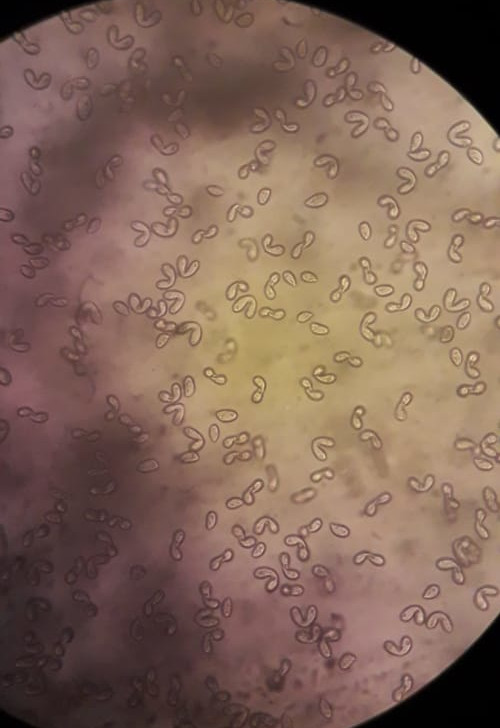
\includegraphics[width=0.6\textwidth]{images/conjugation1.jpeg}
	\caption{Conjugation}
	\label{conjugation1}
\end{figure}

\section{Agarose-Gel}
For 100ml of agarose gelcast of 0.8%, it takes 0.8g of agar and 100ml fo 1x TAE( It's a buffer)
\begin{enumerate}
	\item Tape the gel caste tray
	\item Put the comb on the end of the cast tray
	\item Agar(0.8g)+ 1x TAE(100ml) in a flask
	\item Oven it till dissolution (In this case it took about 5 minutes), check after every minute or so.
	\item Let the flask cool before putting in ETB, but don't let it cool so much as to start polymerization.
	\item Put in EtBr(20\textmu{}l) shake well.
	\item Put it in the tray
	\item Move the bubbles away from the well, towards the ends.
\end{enumerate}

\section{Cell Fixation}
Cell fixation is the process of arresting the cells completely till the protein level. This can be done in two ways.
\begin{enumerate}
	\item PFA

		Paraformaldehyde. The sample of cells are centrifuged to precepetate, the floating part is thrown away, PFA is added quickly. After sometime the cells are suspended again, to the original concentration.
	\item Cooling

		This process involves slow cooling down of the cells.
\end{enumerate}

\section{DAPI Staining}
 4,6-diamidino-2-phenylindole(DAPI) staining is the process of arresting the cells and staining them with a UV Sensitive dye(DAPI).
\begin{enumerate}
	\item Centrifuge 1ml of cell under 1.1G for 2 minutes and discard the supernatant(the floating stuff).
	\item PFA 500\textmu{}l(At the time when you want to arrest them)(In our case at 8 hours for when they were kept together).
	\item Tap and Invert.
	\item Centrifuge under 1.1G for 2 minutes and discard the supernatant(the floating stuff).
	\item Add 200\textmu{}l of 10mM Hepes(A buffer), tap and Invert.
	\item Centrifuge under 1.1G for 2 minutes and discard the supernatant(the floating stuff).
	\item Add 200\textmu{}l of DAPI.(Preferabely in dark)
	\item Leave in dark for 10 minutes.
	\item Centrifuge under 1.1G for 2 minutes and discard the supernatant(the floating stuff).
	\item Take 5\textmu{}l of cells and prepare slide.
\end{enumerate}
DAPI is light sensitive so stored in darkness in fridge.

\end{document}
